


%%\section{Introduction}

%%\label{sect:introduction}



\section{The elusive object}

Sensory information is intrinsically ambiguous, and very distant from
the world of well-defined objects in which humans believe they live.
What criterion should be applied to distinguish one object from
another?  How can perception support such a phenomenon as
figure-ground segmentation?  Consider the example in
Figure~\ref{fig:number-cross}.
%
\begin{figure}[tbh]
\begin{center}
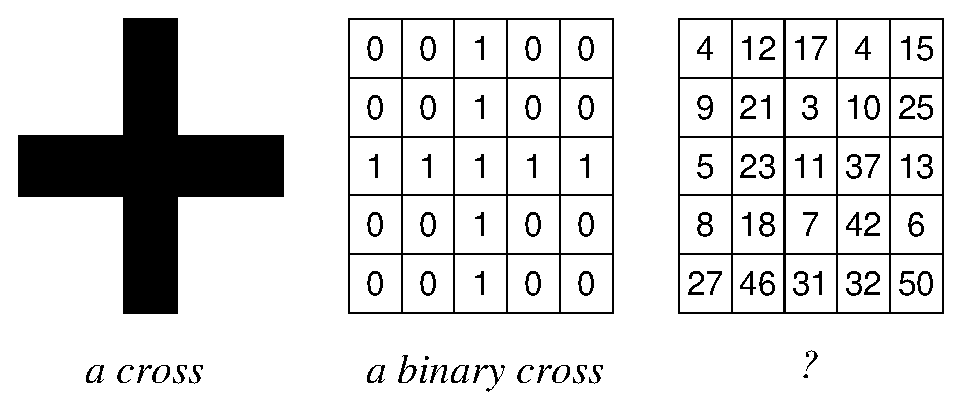
\includegraphics[width=6.5cm]{number-cross.eps}
\caption{ 
\label{fig:number-cross}
%
Three examples of crosses, following \cite{manzotti01coscienza}.  The
human ability to segment objects is not general-purpose, and improves
with experience.
%
}
\end{center}
\end{figure}
%
It is immediately clear that the drawing on the left is a cross,
perhaps because we already have a criterion, which allows segmenting
on the basis of the intensity difference. It is slightly less clear
that the zeros and ones on the middle panel are still a cross. What
can we say about the array on the right?  If we are not told, and we
do not have the criterion to perform the figure-ground segmentation,
we might think this is just a random collection of numbers. But if we
are told that the criterion is ``prime numbers vs. non-prime'' then a
cross can still be identified.

While we have to be inventive to come up with a segmentation problem
that tests a human, we don't have to go far at all to find something
that baffles our robots.  Figure~\ref{fig:setup-sequence} shows a
robot's-eye view of a cube sitting on a table. At first glance this
seems simple enough, but many rules of thumb used in machine vision
for automatic object segmentation fail in this particular case.  And
even an experienced human observer, diagnosing the cube as a separate
object based perhaps on its shadow and subtle differences in the
surface texture of the cube and table, could in fact be mistaken --
perhaps some malicious researcher is up to mischief.  The only way to
find out for sure is to take action, and start poking and prodding.
As early as 1734, Berkeley observed that:
%
\begin{quote}
...objects can only be known by
touch. Vision is subject to illusions, which arise from the
distance-size problem... \cite{berkeley72new}
\end{quote}
%
In this paper, we provide support for a more nuanced proposition: that
while it is true that vision is full of illusions, these illusions
evaporate when the robot can reach out and come into contact with
objects -- even if it has no sense of touch!  While certainly touch is
an important sense, we show that simply involving objects in a causal
chain of events initiated by the robot itself is enough to wipe away much
of the ambiguity that will plague a passive observer.

%
\begin{figure}[tbh]
\begin{center}
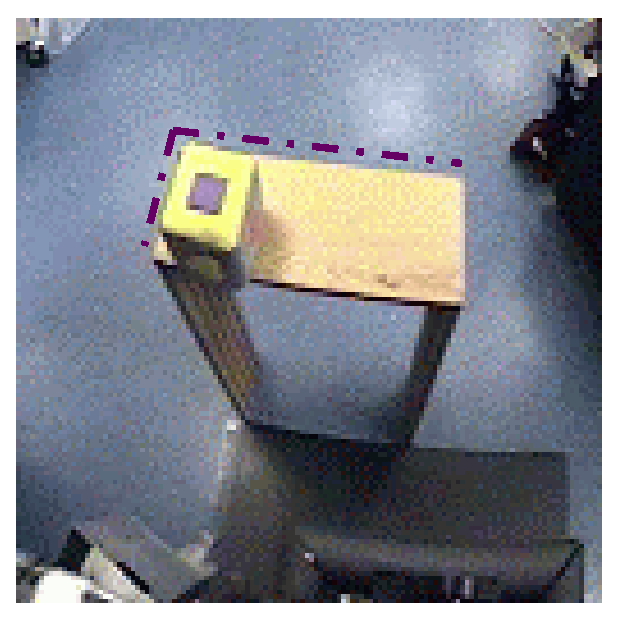
\includegraphics[width=4cm]{setup-sequence.eps}
%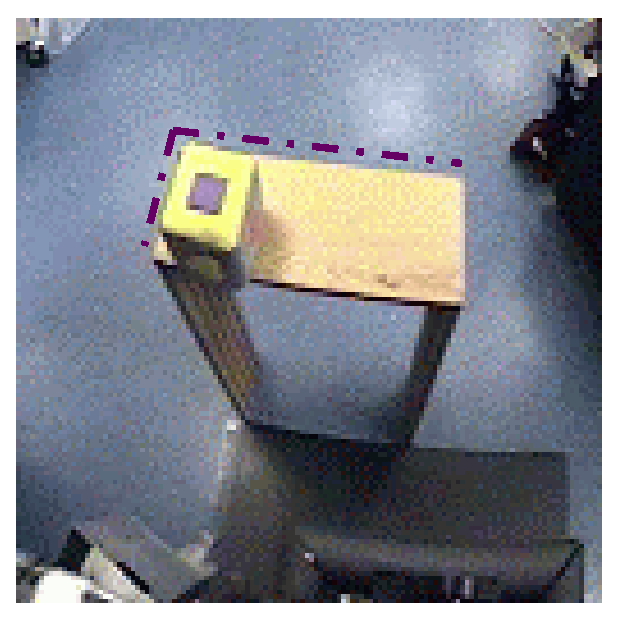
\includegraphics[width=\columnwidth]{setup-sequence.eps}
%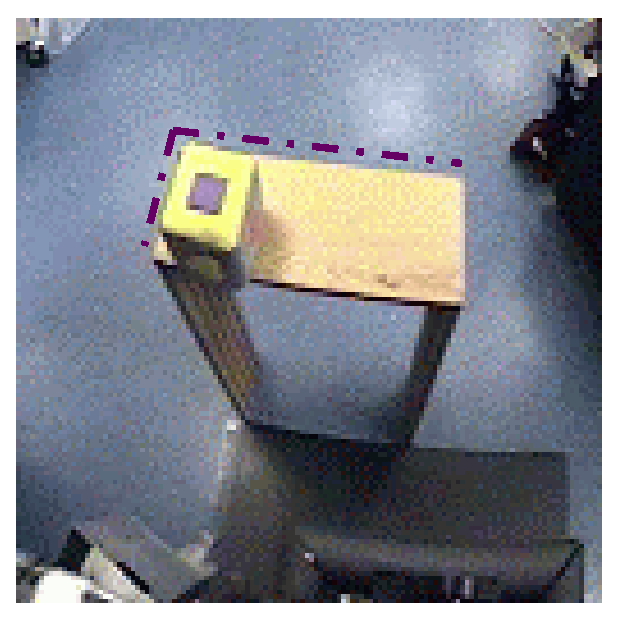
\psfig{file=setup-sequence.eps,width=4cm}
\caption{ 
\label{fig:setup-sequence}
%
A cube on a table. The edges of the table and cube happen to be
aligned (dashed line), the \ahhcolor{}s of the cube and table are not well
separated, and the cube has a potentially confusing surface pattern.
%
}
\end{center}
\end{figure}


\section{Grounding vision in action}

Much of computer vision is passive in nature, with the emphasis on
watching the world but not participating in it.  There are advantages
to moving beyond this to exploit dynamic regularities of the
environment \cite{ballard91animate}.
%%,breazeal00social}.  
A robot has the
potential to examine its world using causality, by performing probing
actions and learning from the response.  Tracing chains of causality
from motor action to perception (and back again) is important both to
understand how the brain deals with sensorimotor coordination and to
implement those same functions in an artificial system, such as a
humanoid robot.  And, as a practical matter, the ability to perform
``controlled experiments'', such as tapping an object lightly, is
crucial to getting to grips with an otherwise complex and uncertain
world.

Figure~\ref{fig:tracing-causes} illustrates three levels of causal complexity
we would like the robot to probe.
The simplest causal chain that the robot experiences is the
perception of its own actions.  The temporal aspect is immediate:
visual information is tightly synchronized to motor commands.
We use this strong correlation to identify parts of the robot
body -- specifically, the end-point of the arm. 

Once this causal connection is established, we can go further and use
it to actively explore the boundaries of objects.  In this case, there
is one more step in the causal chain, and the temporal nature of
the response may be delayed since initiating a reaching movement doesn't
immediately elicit consequences in the environment.  


In this paper, we propose that such causal probing can be arranged in
a developmental sequence leading to a manipulation-driven
representation of objects.  We present results for some important
steps along such a sequence, and describe how we plan to proceed.  We
argue that following this causal chain outwards will allow us to
approach the representational power of ``mirror neurons''
\cite{gallese-fadiga-fogassi-rizzolatti-1996}, where a connection 
is made between our own actions and the actions of another.  

%%As a point of reference, we now
%%briefly review what is known about the relationship of object and
%%action representation in the human brain.

%
\begin{figure}[tbh]
\begin{center}
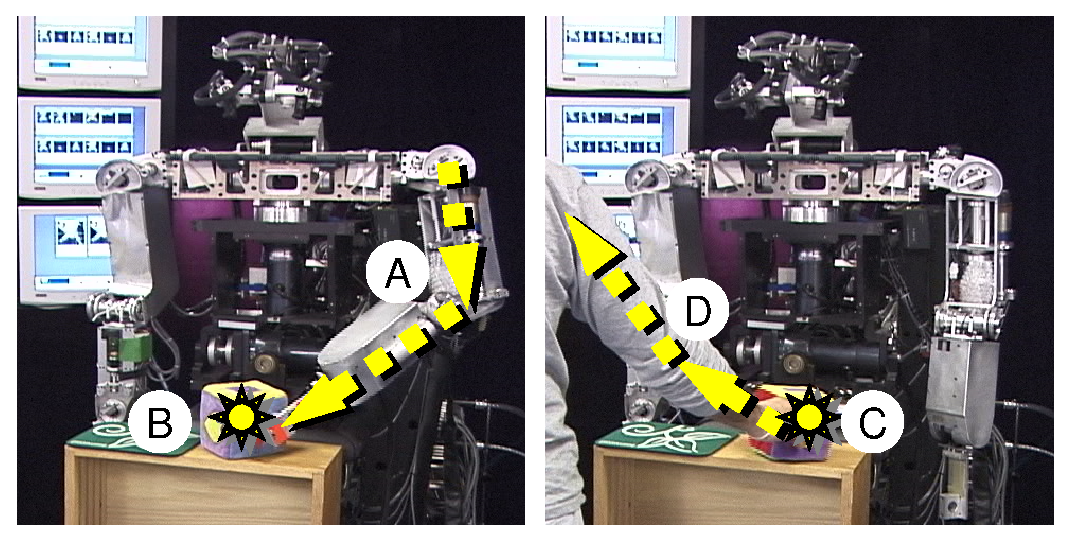
\includegraphics[width=8cm]{tracing_causes.eps}
\caption{ 
\label{fig:tracing-causes}
%
On the left, the robot establishes a causal connection between
commanded motion and its own manipulator (A), and then probes its
manipulator's effect on an object (B).  The object then serves as a
literal ``point of contact'' (C) to link robot manipulation with human
manipulation (on the right, D), as is required for a mirror-neuron-like
representation.
%
}
\end{center}
\end{figure}
%

\section{Objects and actions in the human brain}

The example of the cross composed of prime numbers is a novel (albeit
unlikely) type of segmentation in our experience as adult humans. We
might imagine that in our infancy, we had to initially form a set of
criteria to solve the object identification/segmentation problem
in more mundane circumstances.  We ask the question of whether we can
discover these criteria during ontogenesis.

Humans and a small number of other primates are unique in their
ability to manipulate their environment using tools.
Our capacities are mirrored in the brain by the size of
the cortex controlling them.  Neuroscience has shown that our brains
possess large cortical areas devoted to the control of manipulation --
not surprising, given that encephalization is believed to have evolved
for the purpose of adaptively controlling
action \cite{maturana98tree}.

A useful conceptual schema holds that visual information follows two
distinct pathways in the brain, namely, the dorsal and the ventral
\cite{ungerleider82two,milner95visual}.
The dorsal
pathway controls action directly and pragmatically; conversely, the
ventral takes care of more conceptual skills such as object
recognition.
Of course it is important to remember, when making this dichotomy,
that the two pathways are not completely segregated but rather
complement each other and interact in different
ways \cite{jeannerod97cognitive}.

%%This concept of two distinct visual systems was initially proposed by
%%\cite{ungerleider82two}
%%and successively
%%refined by 
%%Milner and Goodale
%%\cite{milner95visual}. 

Objects are thought to maintain a double ``identity'' depending on
whether they are used in perceptual or in motor tasks. The concept of
size, for example, might be represented multiple times in different
brain areas. Observation of agnosic
patients \cite{jeannerod97cognitive} shows an even more complicated
relationship than the simple dorsal/ventral dichotomy would
suggest.  Although some patients could not grasp generic objects
(e.g. cylinders), they could correctly preshape the hand to grasp
known objects (e.g. a lipstick); interpreted in terms of the
two-pathway system, this implies that the ventral representation of
the object can supply the dorsal system with size information. What we
consciously perceive as ``size'' is rather a collection of different
percepts interacting in a complicated way, and under pathological
circumstances they can be separated from each other. One of the
``identities'' of objects is thus connected to motor performance.

That such pathways develop and are not completely innate is suggested
by the results of \cite{kovacs00human}. She has shown that
perceptual grouping is slow to develop and continues to improve well
beyond early childhood (14 years). Long-range contour integration was
tested and this work elucidated how this ability develops to enable
extended spatial grouping. These results further suggest that the
development of action might precede that of categorization: it is well
established that by 4 months of age infants can process complex
motion stimuli, depth, and \ahhcolor{}.  Roughly at the same age reaching
becomes more consistent.  That is, action comes first
supported by the pragmatic use of diverse sensory modalities;
perception conversely is a long developing process. More studies are
needed though to ascertain how the dorsal pathway (action) influences
the ventral (perception) both in situations like those
already mentioned, and during ontogenesis.

%%%CHANGE%%%
Drawing more from the neural science literature, the results of Fogassi et al.
\cite{fogassi96coding} and Graziano et al. \cite{graziano-hu-gross-1997} have 
shown the existence of neurons that respond to objects and are related to the
description of the peripersonal space with respect to reaching (area F4 and VIP).
A subset of the F4 neurons has a somatosensory, visual, and motor receptive
field. The visual receptive field extends in 3D from a given body part, such
as the forearm. The somatosensory receptive field is usually in register with
the visual one. Motor information is integrated into the representation 
by maintaining the receptive field anchored to the corresponding body part
(the forearm in this example) irrespective of the relative position of the
head and arm. F4, together with areas in the parietal lobe, is thought to 
participate in the visual to motor transformations required to control 
reaching.

While F4 is concerned with the proximal muscles (i.e. reaching), F5
controls more distal muscles (i.e. the hand). Areas in the parietal 
lobe, such as AIP, also project to F5 in the premotor cortex.
For many years the premotor cortex was considered
just another big motor area. New studies (see \cite{jeannerod97cognitive} for a review) 
have demonstrated that this is not the case. We have already described the
properties of the neurons in F4; similarly, researchers have 
identified neurons in the area F5 of the frontal cortex \cite{fadiga00visuomotor} 
that are activated in two situations: {\it i)} when acting onto an object 
(e.g. grasping), and {\it ii)} when looking at the same object (visual response). 
Their firing pattern is quite specific, building a link between the size 
and shape of the object and the applied grasp type (e.g. a small object 
requires a precision grip). These neurons are called canonical. At the time,
this was quite an astonishing discovery because area F5 was believed 
to be only a motor area. A possible interpretation is that the brain 
stores a representation of objects in motor terms, and uses these 
representations to generate an appropriate response to objects. 
Arbib and colleagues \cite{fagg-arbib-1998} interpreted
these responses as the neural analogue of the affordances of Gibson 
\cite{gibson77theory}. In Gibson's theory an affordance is a visual
characteristic of an object which can elicit an action without necessarily
involving an object recognition stage. It seems that areas AIP and F5 are 
active in such a way to provide the individual with a mechanism to 
detect affordances. F5 projects to the primary motor cortex and can 
therefore control \ahhbehavior{}.

\ifverbose
The dorsal stream connects the parietal lobe to the premotor cortex,
which project heavily onto the primary motor cortex to eventually
control movements.
\fi

The gap from object manipulation to hand gesture production and 
recognition is small.
Rizzolatti and coworkers \cite{gallese-fadiga-fogassi-rizzolatti-1996}
extensively probed area F5. They found another class of grasping
neurons that also respond during observation of somebody else's action.
A typical cell of this class (called mirror neuron) indeed responds in two
situations: {\it i)} when executing a manipulative gesture, and {\it
ii)} when observing somebody else executing the same action. These
neurons provide a link between the observation of somebody else's
and our own actions. The activation of F5 is coherent with the idea
that the brain internally reproduces/simulates the observed actions.
Beside the recognition of manipulative actions, mirror neurons are 
thought to support imitative \ahhbehavior s. An intriguing theory
proposed by Rizzolatti and Arbib \cite{rizzolatti98language}
associates mirror neurons to language.

In \cite{wohlsclager02human} the role of objects during an imitative 
task was tested. Also, Woodward \cite{woodward98infants} investigated the role 
of objects in the understanding of action performed by others. In a series 
of experiments she elucidated the contribution that seeing an object 
makes for 5, 6, and 9 month old infants. Taken together, these results provide 
evidence that the object and the goal-directeness of the action represent 
an important component in the understanding of the intentions of others.

%% and to the motor theory of language.

\ifverbose
Another important class of neurons in premotor cortex is found in area
F4 \cite{fogassi96coding}. While F5 is more concerned with the distal
muscles (i.e. the hand), F4 controls more proximal muscles
(i.e. reaching). A subset of neurons in F4 has a somatosensory, visual
and motor receptive field. The visual receptive field (RF) extends in
3D from a given body part, for example, the forearm. The somatosensory
RF is usually in register with the visual one. Finally, motor
information is integrated into the representation by maintaining the
RF anchored to the correspondent body part (the forearm in this
example) irrespective of the relative position of the head and arm.
\fi

\ifverbose
The dorsal/ventral dichotomy is of course a gross simplification of
the reality.  There are neurons in area STS (superior temporal sulcus,
which is a ventral area) that respond to the sight and specific
posture of the hand. They are quasi-mirror neurons but they lack the
motor component (they do not fire in the dark).  Area STS is supposed
to provide the visual information about the posture of the hand to F5
[CITE].
\fi

\ifverbose

\section{Robots and vision}

In the light of these results, we see at least two reasons why
intelligence needs to be embodied. First, if robots are to tell us
something about the functioning of our brains, we have to study its
development in the proper setting, that is, with the robot acting in
the environment. As we have seen action is fundamental to a set of
highly cognitive skills including imitation and language. Perceptual
tasks are also be influenced by action. Second, to build better
robots, adaptive to their environment, there is probably no
alternative but to build them following to some extent biological
principles. The same constraints encountered by biological agents
during ontogenesis are encountered by the robot during its simulated
development.

Certainly, vision and action are intertwined at a very basic level.
While an
experienced adult can interpret visual scenes perfectly well without
acting upon them, linking action and perception seems crucial to the
developmental process that leads to that competence.  We can construct
a working hypothesis: that action is required to object recognition in
cases where an agent has to develop categorization autonomously.  Of
course in standard supervised learning action is not required since
the trainer does the job of pre-segmenting the data by hand.  In an
ecological context, some other mechanism has to be provided.
Ultimately this mechanism is the body itself that through action
(under some suitable developmental rule) generates informative
percepts.

Neurons in area F4 are thought to provide a body map useful for
generating arm, head, and trunk movements. Our robot learns
autonomously a crude version of this body map by fusing vision and
proprioception.  As a step towards establishing the kind of visuomotor
representations seen in F5, we then develop a mechanism for using
reaching actions to visually probe the connectivity and physical
extent of objects without any prior knowledge of the appearance of the
objects (or indeed of the arm itself).

\fi


\section{Robots and Vision}

A vision system is said to be {\em active} if it is embedded within a
physical platform that can act to improve perceptual performance.  For
example, a robot's cameras might servo a rapidly moving target to
stabilize the image and keep the target in view.  In fact, active
vision is often equated with moving cameras, although in this paper we
use it in a broader sense of any controllable resource recruited to
serve vision (including, in our case, arm motion).

Historically, a number of logically distinct ideas are often
associated with active vision.  The first is that vision should be
approached within the the context of an overall task or
purpose~\cite{aloimonos87active}.  If an observer can engage in
controlled motion, it can integrate data from frame to frame to solve
problems that are ill-posed statically.  Well-chosen motion can
simplify the computation required for widely studied vision problems,
such as stereo matching~\cite{bajcsy88active,ballard91animate}.  These
interwoven ideas about active vision are teased apart
in~\cite{tarr94computational}.


Pending citations: \cite{tsikos91segmentation}.

